\section*{Goldponsor und Aussteller}
\begin{flushright}
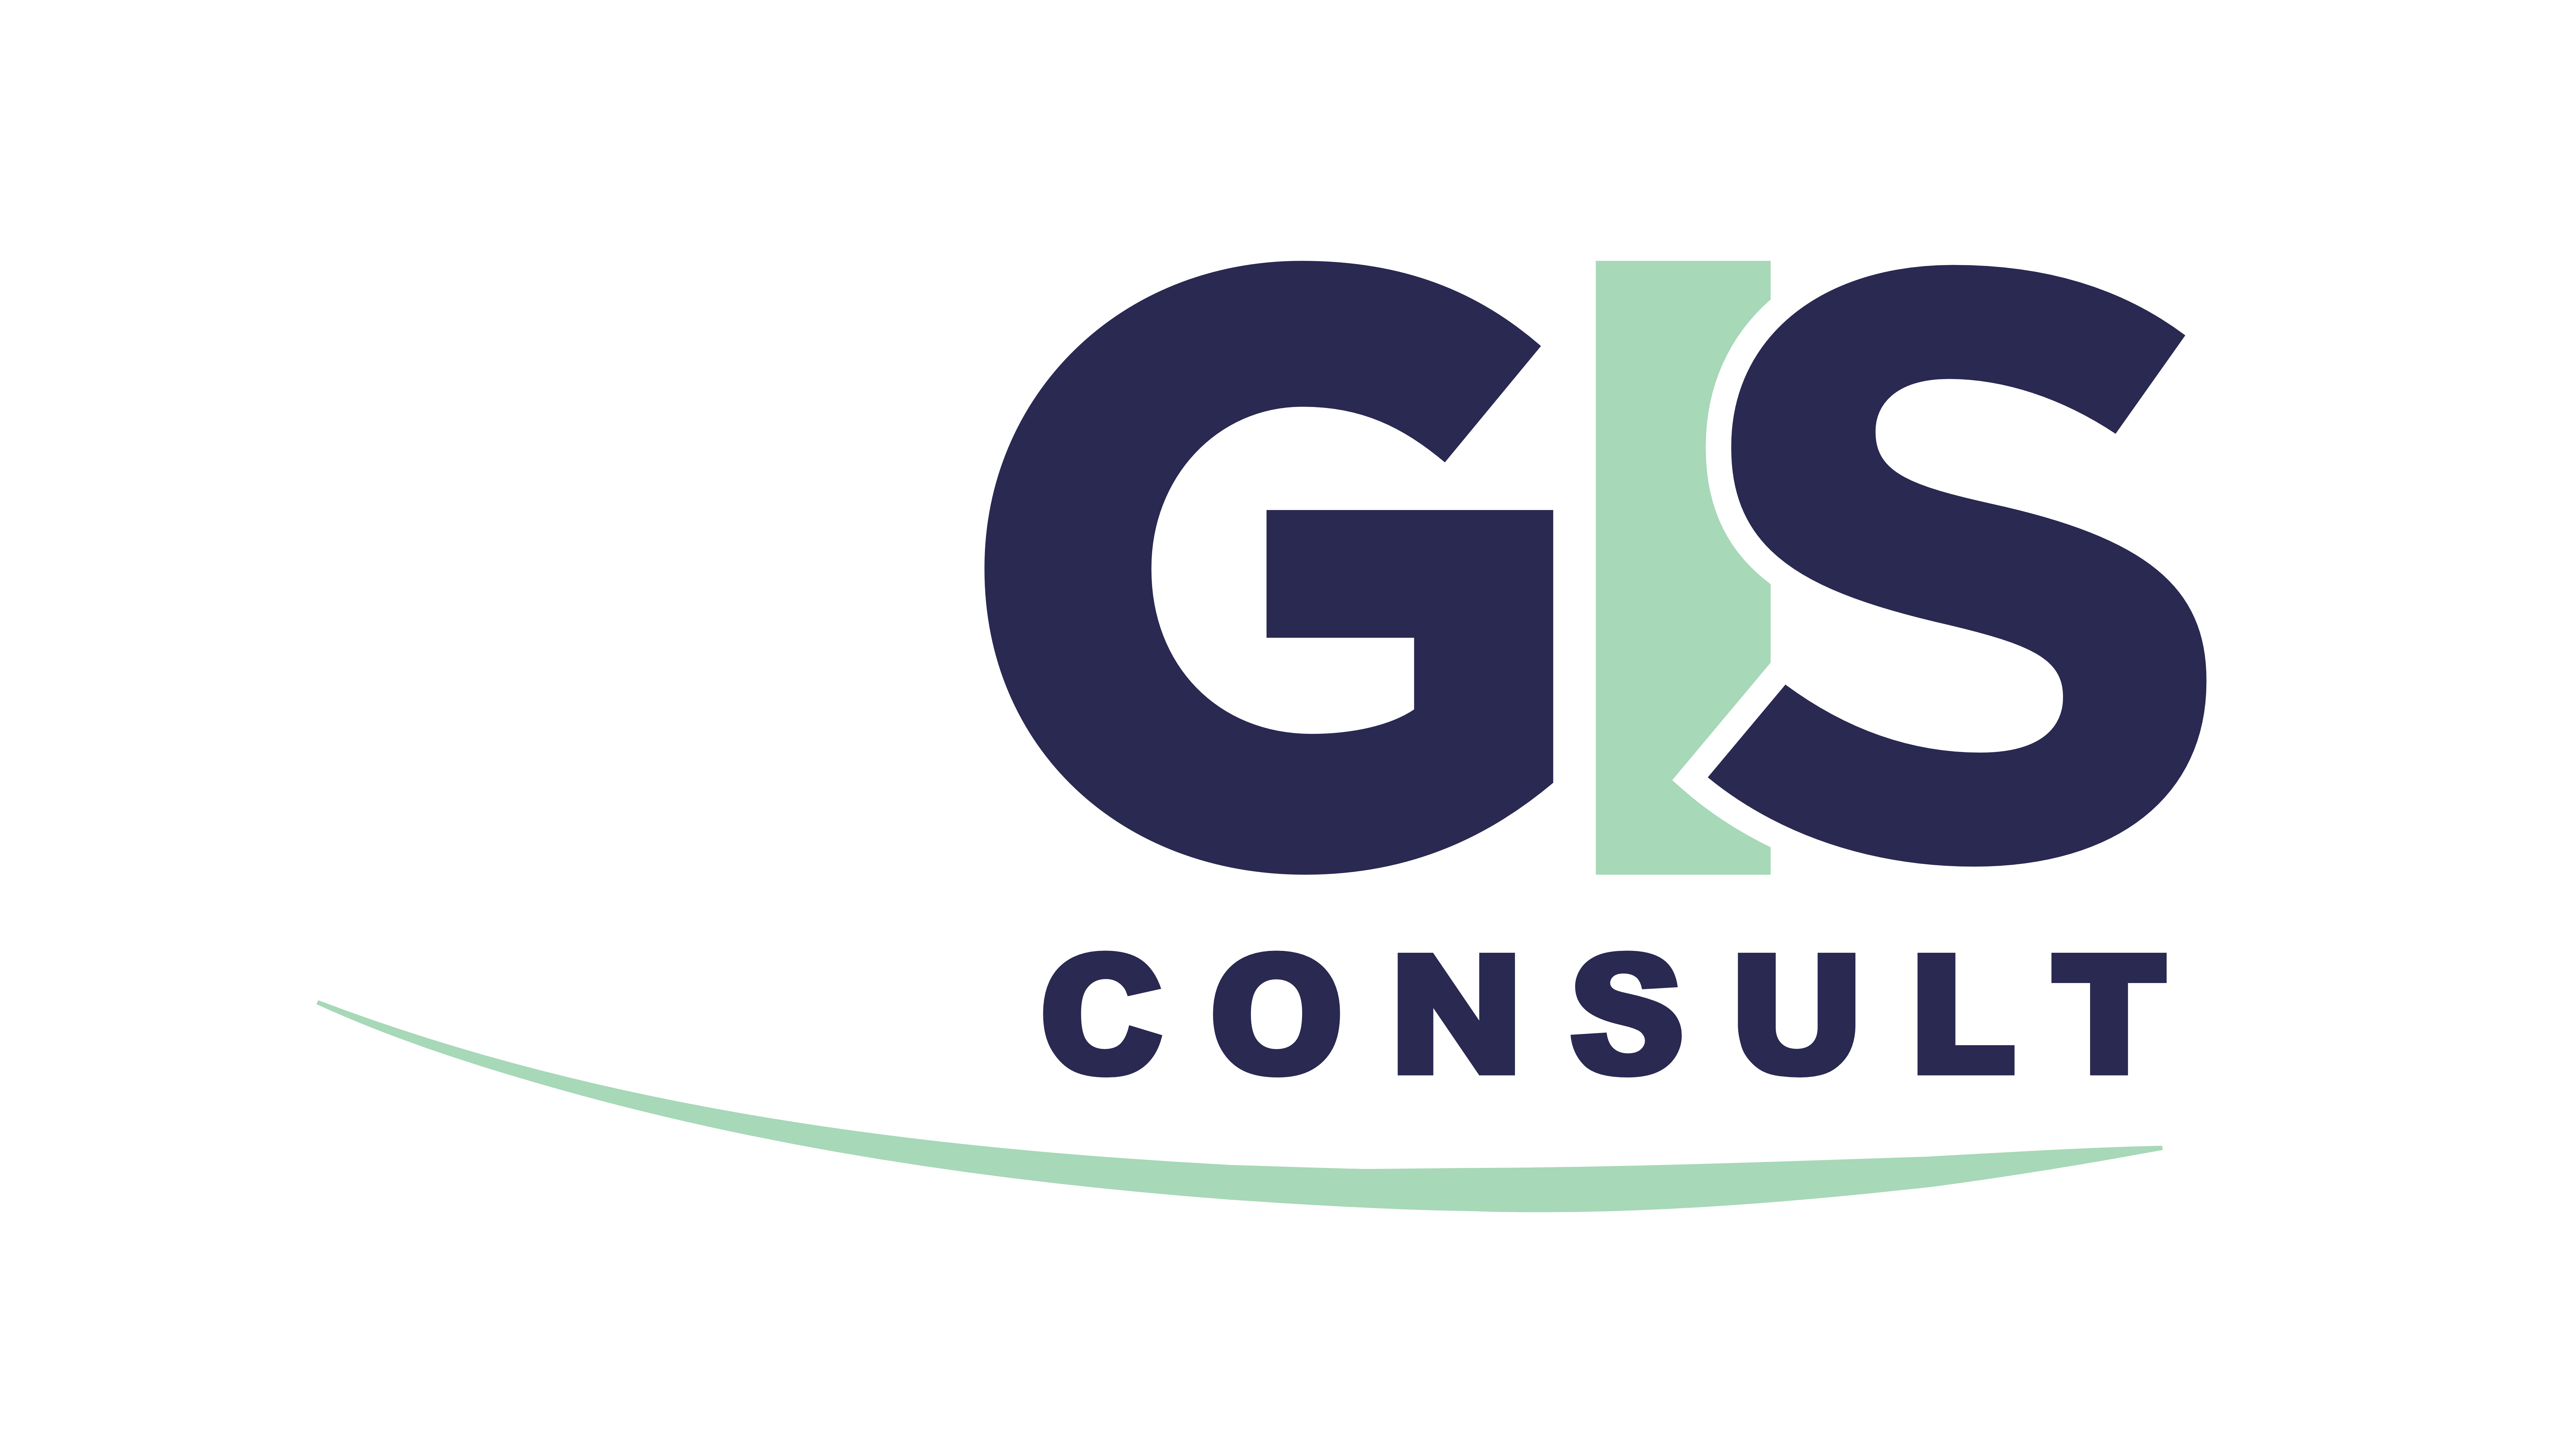
\includegraphics[width=0.7\textwidth]{103_GIS-Consult_Logo.png}
\end{flushright}
\noindent
Die {\bfseries GIS Consult} ist Ihr Partner für nachhaltige Geodatenlösungen. Der Kunde steht bei uns im Mittelpunkt. Seit über 10~Jahren entwickeln wir individuelle Lösungen basierend auf Open-Source, die perfekt auf die Kundenbedürfnisse abgestimmt sind. 

\noindent
Die GIS Consult agiert als Multiplikator für den Einsatz von Open Source. Wir setzen uns aktiv dafür ein, das Bewusstsein für die Vorteile offener Technologien zu stärken und den Einsatz von Open-Source-Lösungen zu fördern.

\noindent
Wir verstehen Open Source als Schlüssel zu Innovation, Transparenz und Nachhaltigkeit. Durch die Nutzung und Weiterentwicklung bewährter Technologien fördern und schaffen wir offene Standards und bieten flexible, zukunftssichere Lösungen.

\noindent
Unser Angebot umfasst Beratung, Implementierung, Schulungen sowie Wartung, Support und Hosting. Von Geoportalen über Planauskünfte bis hin zu Infrastrukturkatastern liefern wir Lösungen für den kommunalen Bereich.

\noindent
Die GIS Consult ist in Haltern am See, Kiel und Erfurt vertreten.
